%\noindent
\begin{figure*}
\centering
\begin{tabular}{ccc}
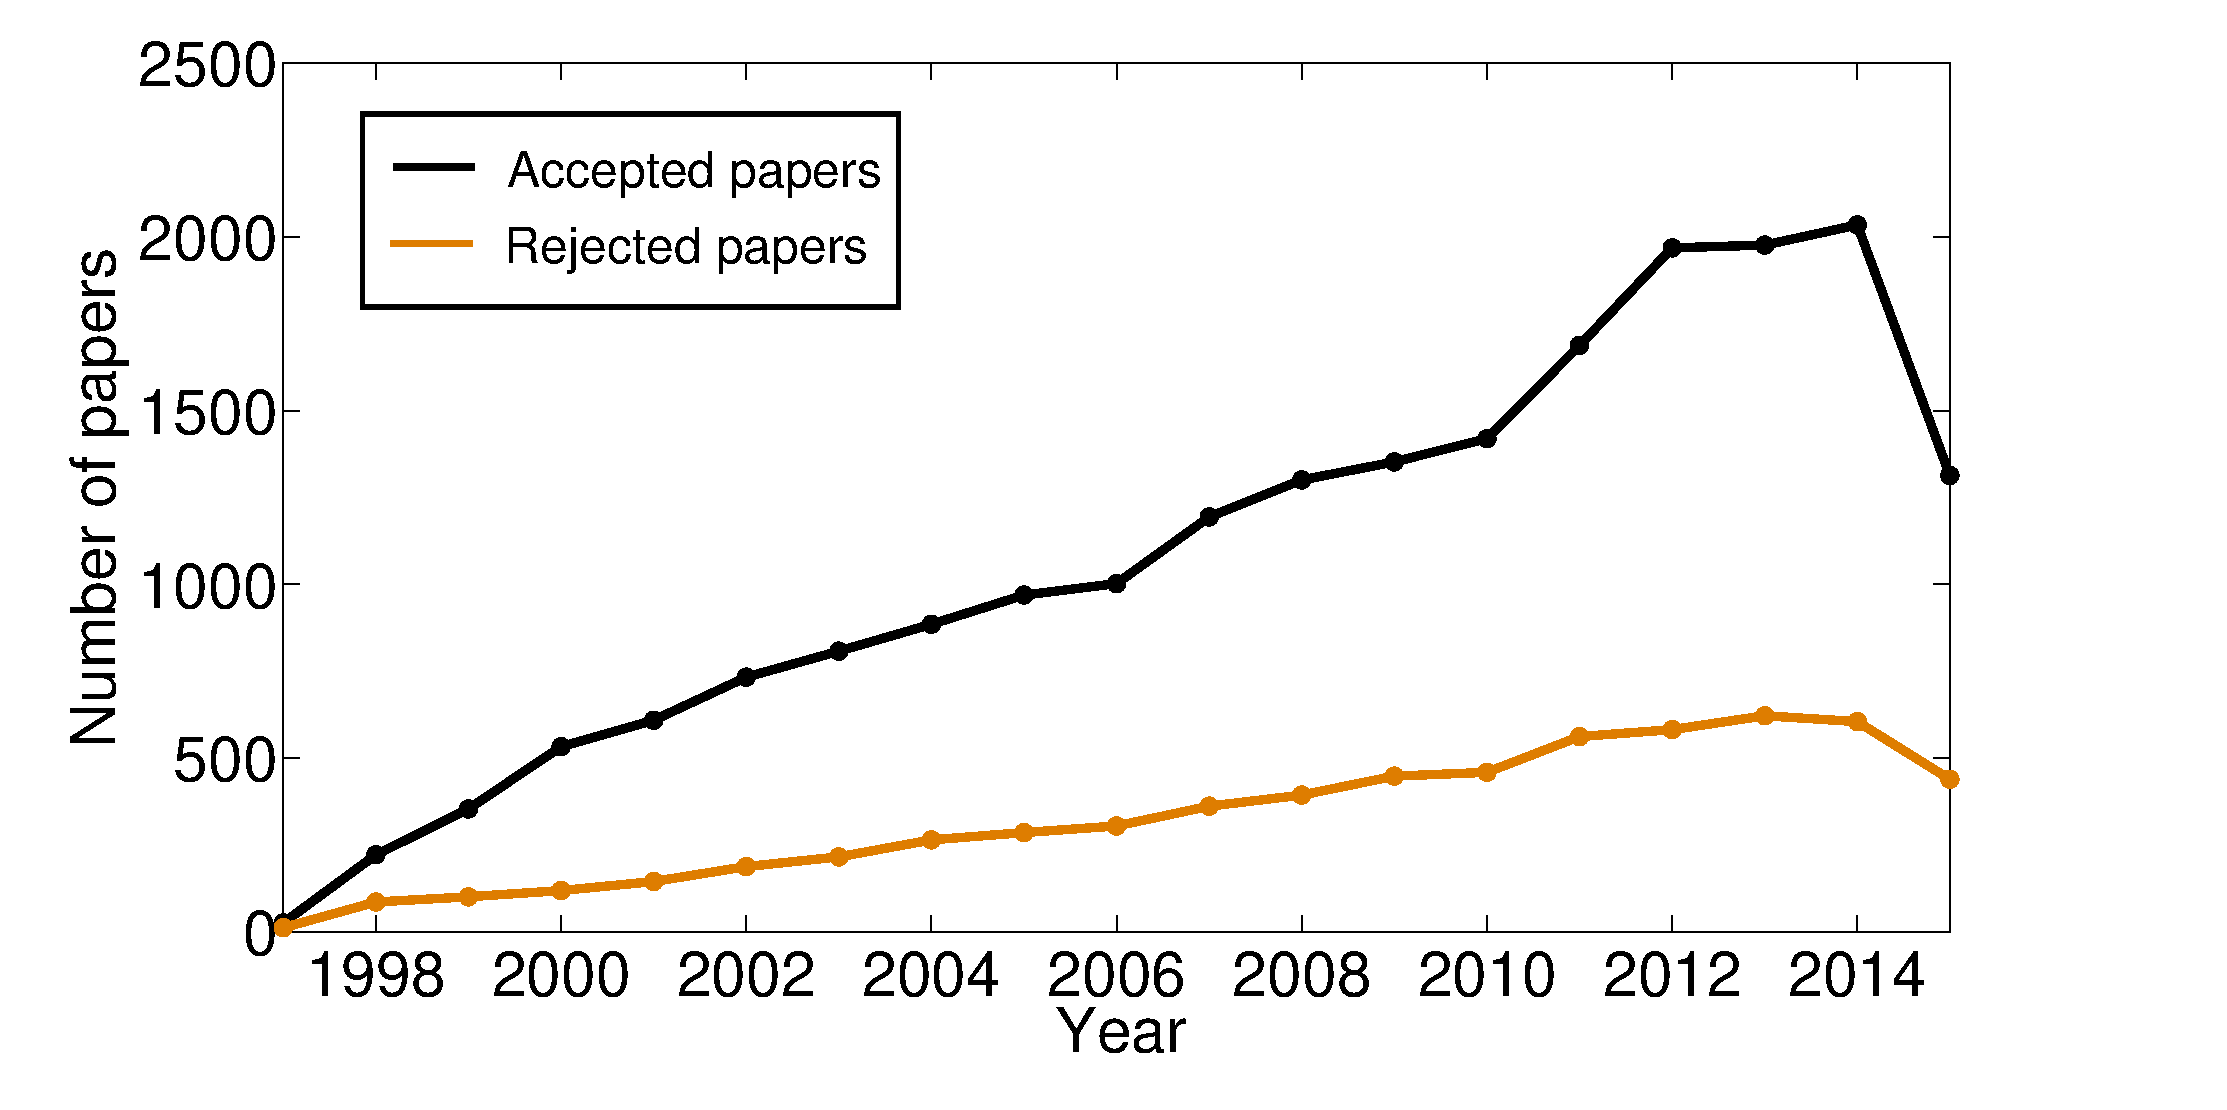
\includegraphics[scale=.12]{./texfiles/Chapter_4/jcdl/figures/paper_year_dis.eps} & 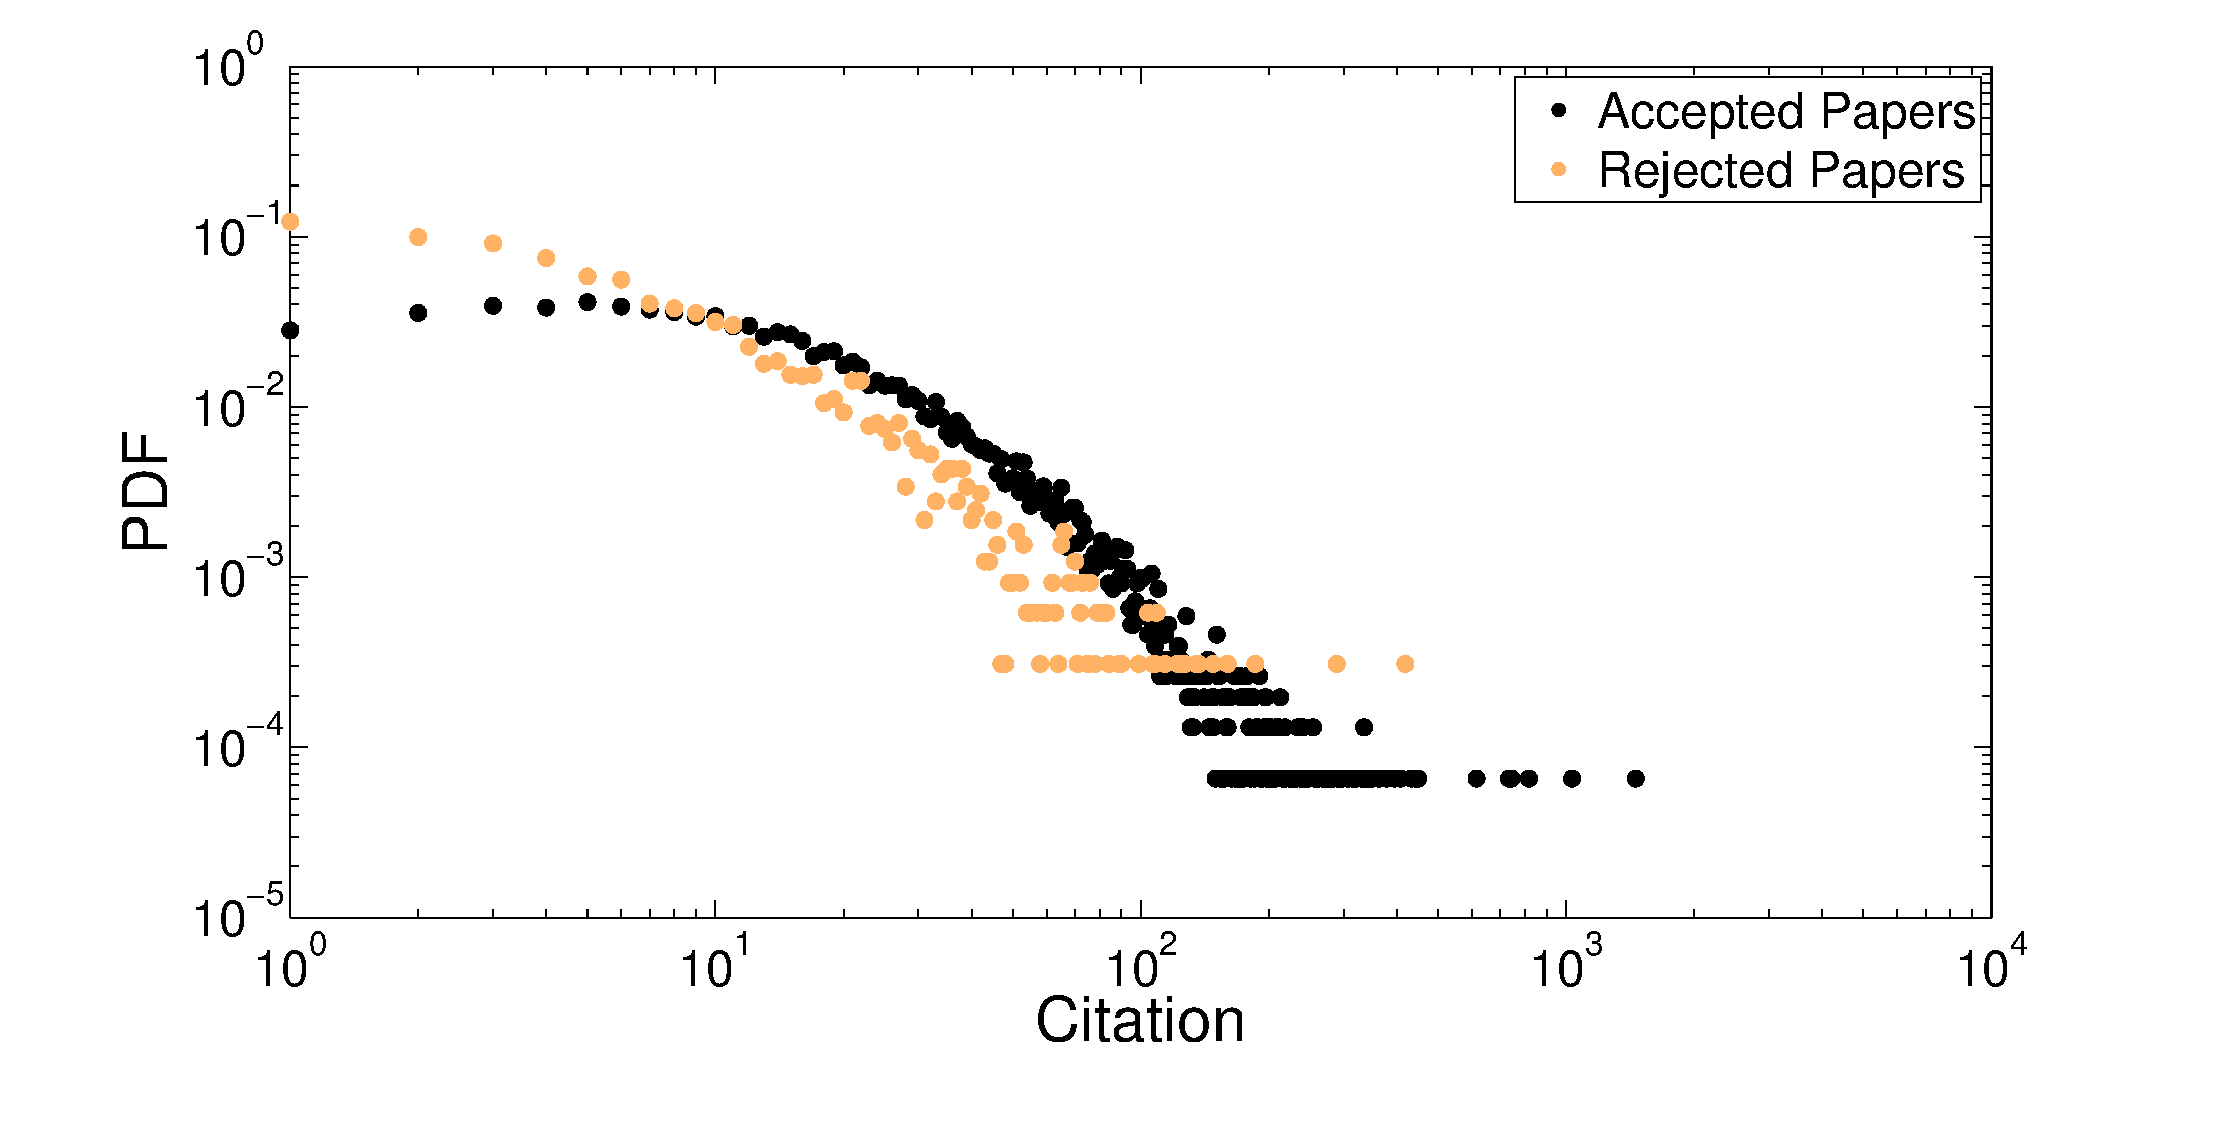
\includegraphics[scale=.12]{./texfiles/Chapter_4/jcdl/figures/citation_distribution.eps} & \includegraphics[scale=0.12]{./texfiles/Chapter_4/jcdl/figures/review_distribution.eps}
\end{tabular}
\caption{{\bf (Left)} Number of accepted and rejected papers per year from 1997 to 2015. {\bf (Middle)} Citation distribution of both the accepted and the rejected papers. {\bf (Right)} Distribution of number of reviews for accepted and rejected papers.}
\label{fig1}
\end{figure*}


The main aim of this work is to understand the importance of the review process and especially the contribution of the referees in this process. Such an analysis requires detailed information of reviews like the number of rounds of review, final decisions and the text of the review report in each round and, lastly, the number of citations for each paper. 

{\em Obtained data:} As stated earlier, for our analysis, we consider the dataset of the {\em Journal of High Energy Physics} (JHEP). It is one of the leading journals in its field and publishes theoretical, experimental and phenomenological papers. Among JHEP's most direct competitors there are Physical Review D, Nuclear Physics, EPJC, Physics Letters B and Physical Review Letters.
This dataset consists of {\bf 28871} papers that were submitted between 1997 (year of inception) and 2015 of which {\bf 20384} were accepted and {\bf 7073} were rejected. The rest of the papers were either withdrawn by the authors or the final decisions were not available. The number of distinct review reports is {\bf 70k} containing {\bf 12m} lines of review text. For each paper we have the title, the abstract, the authors, the date of publication (in case it was accepted) and the number of citations for the accepted papers. The dataset further contains for each paper the number of rounds of reviews it received before it was accepted (rejected) as well as the detailed text of the report submitted by the assigned reviewer and the editor.


\noindent{\em Pre-processing:} To obtain the necessary information for the rejected papers we queried the ``Inspire'' search engine\footnote{\url{https://inspirehep.net}} by their corresponding arXiv\footnote{\url{http://arxiv.org/}} ids. We could obtain for each paper the citation information, the abstract, the title, the authors and also the publishing journal (if at all it got published). Note that all through our analysis we refer to number of citations as the cumulative number of citations that a paper/author obtained at the end of 2015. 
We further had to disambiguate the names of the authors and assign each of them a unique id.  

\noindent{\em Some basic facts about the dataset:} In fig.~\ref{fig1}{\bf(Left)} we plot the year-wise distribution of the accepted and the rejected papers from 1997 to 2015. We observe an increasing trend in the number of submissions except for the year 2015 for which the data is incomplete. 
\begin{table}[htpb]
\centering
\caption{General information of the dataset.}
%\vspace{-2mm}
\label{tab1}
\begin{tabular}{|l|l|}
\hline
Number of papers                                                                 & 28871 \\ \hline
\hline
\begin{tabular}[c]{@{}l@{}}Number of papers (accepted)\end{tabular}            & 20384 \\ \hline
\begin{tabular}[c]{@{}l@{}}Number of papers (rejected)\end{tabular}            & 7073  \\ \hline
\begin{tabular}[c]{@{}l@{}}Average number of reviews (accepted papers)\end{tabular}   & 1.76  \\ \hline
\begin{tabular}[c]{@{}l@{}}Average number of reviews (rejected papers)\end{tabular}   & 1.35  \\ \hline
\begin{tabular}[c]{@{}l@{}}Average number of citations (accepted papers)\end{tabular} & 31.89 \\ \hline
\begin{tabular}[c]{@{}l@{}}Average number of citations (rejected papers)\end{tabular} & 9.45  \\ \hline
\end{tabular}
%\vspace{-2mm}
\end{table}
\begin{figure}
\centering
\includegraphics[scale=0.3]{./texfiles/Chapter_4/jcdl/figures/peer_review.jpg}
\caption{\label{peer_review} Peer-review system in JHEP}
\end{figure}
In fig.~\ref{fig1}{\bf(Middle)} we plot the citation distribution of the accepted and the rejected papers. Both the distributions seem to follow a power-law behavior. We further plot 
the distribution of the number of reviews for the accepted and the rejected papers in fig.~\ref{fig1}{\bf(Right)}. An important observation is that for JHEP, majority of the 
papers undergo one or two rounds of reviews after which they are either accepted or rejected. 
We note certain general information related to the dataset in table~\ref{tab1}.
Each submitted paper in the dataset also consists of the list of authors. There are {\bf 15127} unique authors in the dataset with at least one submission to JHEP and {\bf 12434} authors with at least one accepted paper. The average number of submissions per author is {\bf 5.18} while the number of authors per paper is {\bf 2.87}. 

\noindent{\em Peer-review process in JHEP:} For every submitted paper the administrator assigns an editor for it. The editor selects a single or a small set of reviewers for judging the quality of the contributions in the paper. The reviewer sends back his views in the form of a report. Based on this report the editor decides whether to accept or reject the paper. The editor may also ask the authors to reshape the paper based on the feedback of the reviewer(s) and in which case they have to resubmit before a decision on its acceptance could be taken. In fig.~\ref{peer_review}, we present a schematic showing the peer-review process in JHEP.

\medskip